\chapter{FUNDAMENTAÇÃO TEÓRICA}
Este capítulo apresenta os conceitos que sustentam o desenvolvimento deste estudo. Primeiramente, examinam-se os fundamentos de \gls{ia}, \gls{pln} e modelos de linguagem, incluindo a arquitetura \textit{Transformer} e a técnica de \gls{rag}, que formam a base técnica do sistema proposto. Em seguida, descreve-se a estratégia de automação inteligente aplicada à verificação de documentos educacionais, detalhando seu \textit{pipeline}, vantagens e limitações. Na sequência, discutem-se as ferramentas de automação e integração empregadas. Por fim, revisam-se trabalhos relacionados que posicionam esta proposta no contexto da pesquisa sobre \gls{ia} na educação.

\section{Inteligência Artificial, PLN e Modelos de Linguagem}
A \acrlong{ia} constitui o ramo da ciência da computação dedicado a criar sistemas que emulem facetas da inteligência humana, como o raciocínio, o aprendizado e o processamento de informações \cite{RussellNorvig2021}. Nesse domínio, o \gls{pln} se destaca por possibilitar a interação entre máquinas e a linguagem humana, em formatos escritos ou estruturados. O \gls{pln} tem impulsionado avanços em atividades como extração de dados, categorização de textos e reconhecimento de padrões, vitais para a verificação de documentos educacionais \cite{RussellNorvig2021}.

Historicamente, a validação de documentos era realizada por sistemas baseados em regras ou métodos estatísticos limitados. A emergência dos \glspl{llm}, que empregam redes neurais profundas com bilhões de parâmetros e mecanismos de atenção, ampliou essa capacidade. Ao contrário de métodos convencionais, os \glspl{llm} captam contextos elaborados, identificam relações semânticas distantes e produzem textos ou sugestões de modo natural. Entre os exemplos proeminentes estão os modelos da família \gls{gpt}, voltados para a geração de texto, e modelos abertos que podem ser executados localmente. Suas aplicações abrangem desde analisadores textuais até sistemas de verificação automática, formando a base para a automação inteligente de planos de ensino.

\subsection{Arquitetura \textit{Transformer}}
A arquitetura \textit{Transformer} configura um dos avanços mais impactantes no \gls{pln}, servindo como alicerce para os principais modelos de linguagem atuais. Apresentada por \citeonline{Vaswani2017}, essa estrutura substitui as redes neurais recorrentes e convolucionais por um mecanismo de atenção, que identifica conexões semânticas entre palavras em uma sequência, independentemente da posição. O cerne do modelo é o mecanismo de \textit{self-attention}, que permite ao sistema avaliar a importância de cada elemento em relação aos outros em um documento. Esse procedimento cria representações contextuais mais robustas, habilitando a captura de dependências distantes, desafio para arquiteturas prévias.

O \textit{Transformer} compreende duas seções principais: o \textbf{codificador} (\textit{encoder}), que trata a entrada textual e produz representações vetoriais internas, e o \textbf{decodificador} (\textit{decoder}), que usa essas representações para gerar saídas, como propostas de correção. Essa composição modular facilita o treinamento em grandes conjuntos de dados e a aplicação em variadas tarefas, como a classificação de seções de um plano de ensino e a geração de relatórios. Devido a essas qualidades, o \textit{Transformer} tornou-se a base de modelos como o \gls{bert} e o \gls{gpt} \cite{Vaswani2017}. Alternativas anteriores, como as redes \gls{lstm}, uma variação das \gls{rnn}, também capturam dependências sequenciais, mas com maior dificuldade em sequências longas e sem o paralelismo que torna o treinamento do \textit{Transformer} mais eficiente \cite{Vaswani2017}.

\subsection{Limitações dos LLMs e a Técnica RAG}
Quando operados isoladamente, os \glspl{llm} geram análises coerentes a partir do conhecimento absorvido no treinamento. Esses modelos, referidos como \glspl{llm} puros, oferecem fluidez e generalização como vantagens, mas também exibem limitações: ausência de acesso a dados atuais ou específicos de uma instituição, falta de precisão em áreas especializadas e propensão a alucinações, situação em que fornecem informações errôneas com convicção aparente.

Como resposta a essas limitações, \citeonline{lewis2020} propuseram a técnica de \gls{rag}, que combina um modelo gerador com um mecanismo de recuperação de documentos. Antes de produzir a resposta, o sistema consulta uma base de conhecimento externa, tipicamente armazenada como vetores de \textit{embeddings}, e fornece os trechos mais relevantes ao \gls{llm} como contexto. No caso deste trabalho, essa base é composta pelos regulamentos institucionais do \gls{ifc} e pelo \gls{ppc} do curso. Isso atenua alucinações, eleva a confiabilidade e permite adaptação ao contexto educacional, garantindo que a verificação seja fundamentada nos padrões reguladores da instituição, e não apenas no conhecimento genérico do modelo.

\section{Automação Inteligente para Validação de Planos de Ensino}
A \textbf{automação inteligente} destinada à verificação de planos de ensino é formada por componentes-chave: um módulo de extração e pré-processamento de texto, que identifica as seções presentes nos documentos; uma base de conhecimento normativa; e um módulo de análise baseado em \gls{llm} com \gls{rag}, que avalia a conformidade de cada seção e propõe ajustes. Tal configuração permite o tratamento semiautomático de planos de ensino, adequando-os às diretrizes institucionais, como a Organização Didática do \gls{ifc} \cite{ifc2022}.

O processo se desenrola em fases: primeiramente, o documento é convertido em texto estruturado, utilizando \gls{ocr} quando apropriado; em seguida, o texto é segmentado em seções, como ementa, objetivos, metodologia, avaliação e referências; por fim, cada seção é confrontada com os critérios estabelecidos, resultando em relatórios que apontam deficiências. A principal motivação reside na diminuição de inconsistências comuns em processos manuais, mantendo o avaliador humano responsável pela decisão final, conforme recomendado por relatórios de política educacional sobre o uso de \gls{ia} \cite{USDeptEd2023}.

\subsection{Funcionamento do \textit{Pipeline}}
O sistema é organizado para unir módulos de extração, análise e produção de relatórios, funcionando de maneira integrada para converter um plano de ensino em uma análise de conformidade. Na fase de \textbf{extração}, o documento em PDF é convertido em texto e dividido em segmentos correspondentes às seções do plano. Esses segmentos substituem a inspeção manual por uma identificação automática de itens como cronogramas, critérios de avaliação e referências bibliográficas.

Na etapa de \textbf{análise e validação}, o \gls{llm} recebe cada segmento juntamente com os trechos relevantes das normas recuperados pela base de conhecimento (\gls{rag}) e classifica o item como conforme, incompleto ou ausente, gerando uma justificativa e, quando cabível, uma recomendação de correção. Esse procedimento assegura consistência entre avaliações e rastreabilidade das decisões, uma vez que a norma que fundamentou cada apontamento pode ser exibida ao usuário. A Figura \ref{fig:pipeline} apresenta uma visão geral desse fluxo.

\begin{figure}[H]
\centering
\caption{Visão geral do \textit{pipeline} de validação com \gls{llm} e \gls{rag}.}
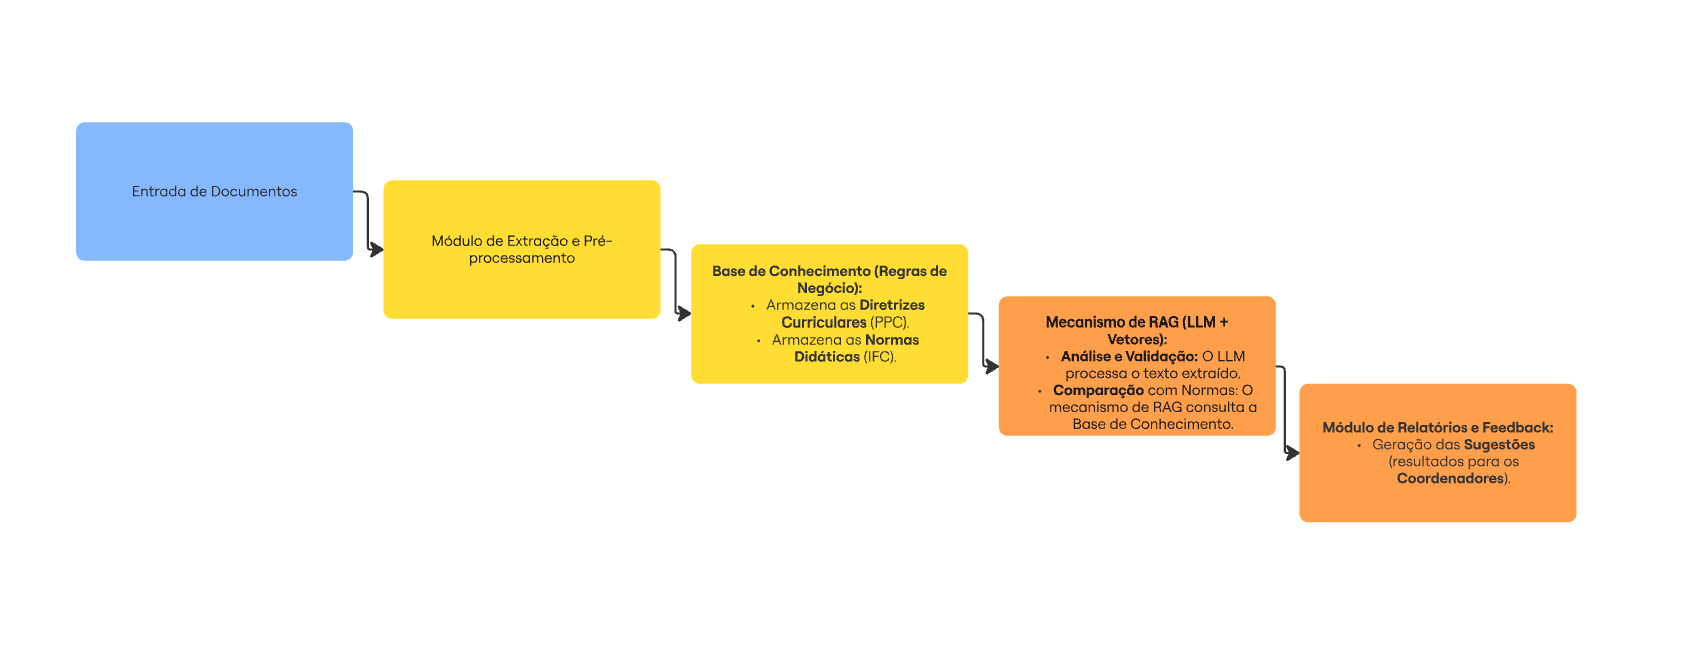
\includegraphics[width=\linewidth]{images/1234567.png}
\label{fig:pipeline}
\legend{Fonte: Elaborado pelo autor.}
\end{figure}

Em resumo, o \textit{pipeline} de um sistema de automação inteligente possibilita a fusão de análise semântica com verificação contextual, entregando resultados ancorados nas diretrizes educacionais da instituição.

\subsection{Vantagens e Limitações}
A estrutura de automação inteligente oferece diversas vantagens em relação à verificação manual. Uma delas é a minimização de inconsistências entre avaliadores, como variações na checagem de referências ou de critérios avaliativos, fomentando maior uniformidade. Outro benefício é a economia de tempo, permitindo que o \gls{nde} se concentre em ações estratégicas, como o refinamento pedagógico, em vez de tarefas rotineiras. Essa qualidade é particularmente valiosa em instituições com grande número de disciplinas, onde a capacidade de expansão é vital. Ademais, o sistema promove a transparência ao exibir as normas empregadas na verificação, possibilitando que os docentes confirmem a procedência das sugestões.

No entanto, a técnica também apresenta restrições. O desempenho do sistema depende da qualidade da base normativa e da capacidade do modelo de interpretá-la. Caso os documentos de entrada sejam inconsistentes ou mal formatados, a extração pode falhar e a verificação resultante refletir essas imperfeições. Além disso, a execução de \glspl{llm} envolve custos computacionais relevantes e requer infraestrutura apropriada, sobretudo quando se opta por modelos locais. Por fim, a revisão sistemática de \citeonline{Tan2025} alerta que a adoção de \gls{ia} por docentes depende de formação adequada, o que reforça a necessidade de manter a decisão final com o avaliador humano.

\section{Ferramentas de Automação e Integração}
A união entre sistemas de \gls{ia} e plataformas de automação demonstra ser uma abordagem eficaz para assegurar escalabilidade, modularidade e manutenção contínua de aplicações. Neste estudo, o Python e plataformas de orquestração de fluxos de trabalho emergem como opções práticas para coordenar as etapas de coleta, tratamento e verificação de documentos educacionais.

Python é uma linguagem versátil que facilita a conexão de serviços e sistemas via \textit{scripts} modulares. Cada fluxo consiste em funções que representam etapas específicas, como o recebimento de um documento, a extração de texto de PDFs, a segmentação por seções ou a chamada a um \gls{llm}. Bibliotecas como spaCy, para \gls{pln}, e PyMuPDF, para manipulação de PDFs, reduzem o esforço de desenvolvimento. Trabalhos anteriores demonstram a viabilidade de aplicar \gls{pln} em Python a conteúdos educacionais em português, como o sistema de recomendação de conteúdo educacional desenvolvido na UFSC \cite{VieiraFilho2024}.

Plataformas de automação de fluxos de trabalho, como o n8n, permitem orquestrar visualmente as etapas do \textit{pipeline}, integrando serviços de armazenamento de arquivos, chamadas a \glspl{api} de \gls{ia} e a gravação de resultados, com \textit{scripts} Python para validações personalizadas. A automação também auxilia no registro e no exame das verificações: é possível registrar cada análise, quantificar processamentos, identificar deficiências recorrentes e gerar relatórios automáticos para o \gls{nde}. Esses registros apoiam a avaliação de desempenho e as decisões sobre expansão ou ajustes.

Ademais, a operação de sistemas com componentes de \gls{ml} em produção exige práticas de \gls{mlops}, que cobrem a qualidade dos dados de entrada, o monitoramento dos modelos e a consistência das saídas ao longo do tempo \cite{Kreuzberger2023}. O emprego dessas práticas visa não só simplificar o gerenciamento técnico, mas também fomentar uma infraestrutura sustentável e replicável, adequada às demandas de instituições educacionais que buscam modernizar suas operações administrativas.

\section{Trabalhos Relacionados}
O emprego de modelos de \gls{ia} para automação de procedimentos administrativos na educação tem sido investigado extensivamente em pesquisas recentes. Esta seção examina estudos que apresentam métodos similares ou tratam de desafios pertinentes ao projeto de sistemas de verificação semiautomática, servindo como comparação para o sistema proposto.

\subsection{Panorama geral: IA na Educação}
A análise bibliométrica de \citeonline{Metli2023}, que examinou 6.498 artigos indexados na Web of Science entre 1984 e 2022, identificou um crescimento anual de 22,68\% nas publicações sobre \gls{ia} e educação. Como mostra a Figura \ref{fig:publicacoes_ia}, a produção anual permaneceu abaixo de 100 artigos até 2014 e acelerou de forma acentuada a partir de 2019, chegando a 2.361 artigos em 2022, quase dez vezes o volume de 2018. Esse crescimento evidencia a consolidação da área e o interesse crescente em aplicações práticas.

\begin{figure}[H]
\centering
\caption{Artigos publicados por ano sobre \gls{ia} e educação (2006--2022).}
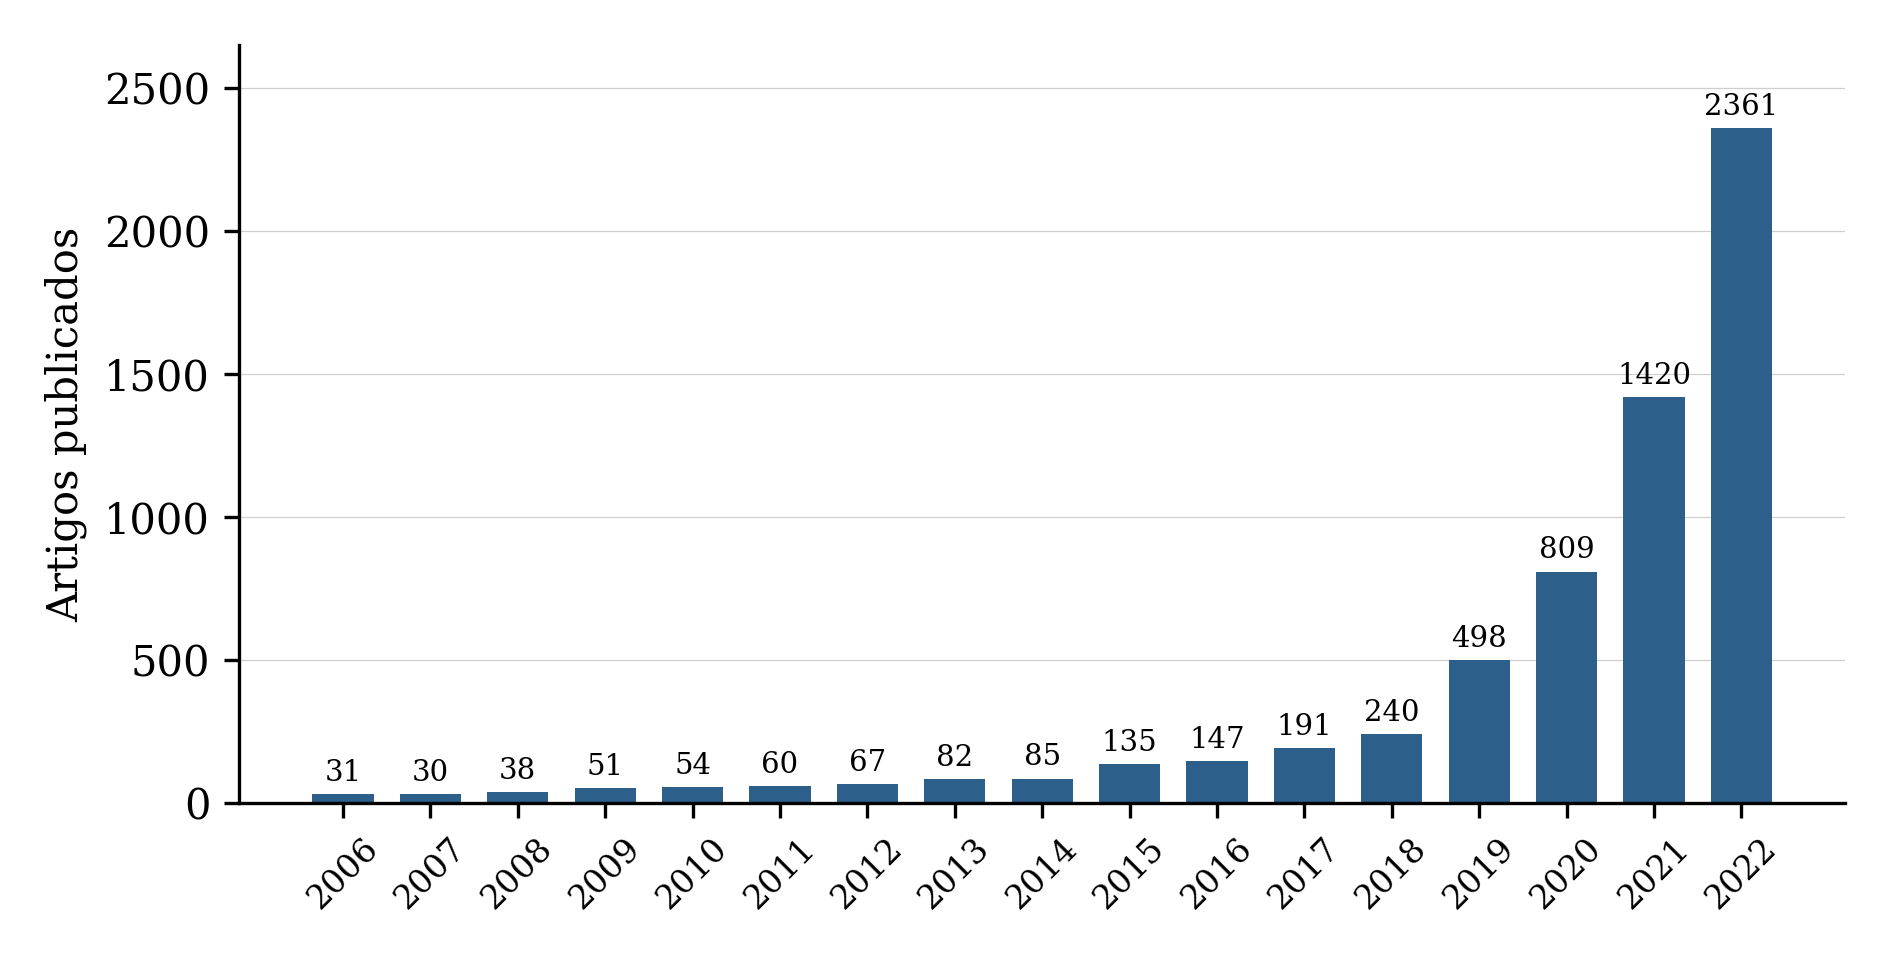
\includegraphics[width=0.9\textwidth]{images/publicacoes_ia_metli.png}
\label{fig:publicacoes_ia}
\legend{Fonte: Elaborado pelo autor com dados de \citeonline{Metli2023}.}
\end{figure}

\citeonline{Tan2025} oferecem uma revisão sistemática sobre o uso de \gls{ia} no ensino e no desenvolvimento profissional de educadores, analisando 95 publicações de 2015 a 2024. Os autores identificam aplicações em apoio ao planejamento de aulas, avaliação automatizada, \textit{feedback} individualizado e otimização de tarefas administrativas, com impactos positivos em eficiência. Contudo, apontam a escassez de estudos sobre a preparação dos docentes para o uso dessas ferramentas e sobre aplicações em processos administrativos de instituições de ensino superior, como a verificação de documentos pedagógicos. Essa lacuna enfatiza a necessidade de pesquisas que investiguem o potencial da \gls{ia} na gestão administrativa educacional, onde este trabalho se posiciona.

\subsection{Aplicação empírica de IA no apoio ao ensino}
\citeonline{Hoare2025} relatam a experiência do Departamento de Educação de Nova Gales do Sul, na Austrália, que desenvolveu uma ferramenta própria de \gls{ia} generativa, o NSWEduChat, testada em 50 escolas a partir de 2024 para apoiar práticas de ensino baseadas em evidências. Entre os mais de 100 professores que participaram da formação associada, 95\% afirmaram que o uso da ferramenta economizaria tempo e todos a recomendariam a colegas. O estudo destaca que a principal vantagem reside na contextualização das respostas com base em materiais e diretrizes institucionais, o que eleva a confiança dos docentes nos resultados. Essas observações apoiam a relevância de abordagens similares, fundamentadas em documentos normativos, em contextos institucionais como o do \gls{ifc}.

\subsection{IA na gestão educacional brasileira e nos Institutos Federais}
No contexto nacional, \citeonline{Santos2025} analisam a adoção de plataformas digitais e de \gls{ia} na gestão das redes públicas de ensino e das escolas. Os autores identificam ganhos na personalização de processos e na organização do trabalho administrativo, mas alertam que a centralização dessas plataformas pode restringir a autonomia dos atores escolares. Concluem que uma adoção responsável exige transparência no uso dos dados, formação continuada e infraestrutura adequada, condições que reforçam a opção deste trabalho por um sistema semiautomático, com modelo executado localmente e decisão final humana.

Especificamente sobre a rede federal, \citeonline{Vieira2025} realizam uma revisão integrativa das experiências com \gls{ia} nos Institutos Federais e constatam pouca produção acadêmica sobre o tema, concentrada nas regiões Sudeste e Nordeste. Entre as quatro formas de incorporação identificadas, a \gls{ia} como apoio administrativo aparece como a menos explorada. Essa constatação evidencia a lacuna que este trabalho busca preencher ao aplicar \gls{ia} a um processo administrativo de um Instituto Federal da região Sul.

\subsection{Considerações Finais sobre os Trabalhos Relacionados}
A revisão dos estudos relacionados destaca a consolidação de técnicas de \gls{ia} em diversos domínios educacionais, com ênfase no potencial para aprimorar a eficiência administrativa. \citeonline{Tan2025} traçam o panorama geral da \gls{ia} na educação e apontam a lacuna em processos administrativos, enquanto \citeonline{Hoare2025} demonstram empiricamente a aceitação de ferramentas fundamentadas em diretrizes institucionais. \citeonline{Sposato2025} sistematiza as aplicações de \gls{ia} na gestão educacional, incluindo a automação de análises documentais. No Brasil, \citeonline{Santos2025} discutem as condições para uma adoção responsável na gestão pública de ensino e \citeonline{Vieira2025} confirmam a escassez de experiências com \gls{ia} como apoio administrativo nos Institutos Federais.

Nenhum dos trabalhos revisados, contudo, trata especificamente da validação de planos de ensino frente a normas institucionais. Frente a essa lacuna, este trabalho aplica a automação inteligente com \gls{llm} e \gls{rag} ao contexto do \gls{ifc}, com ênfase na verificação semiautomática de planos de ensino, buscando fornecer uma solução acessível, confiável e alinhada às necessidades administrativas de docentes e coordenadores, contribuindo para a transformação digital no ensino superior público.
